%!TEX root = ../main.tex

\setcounter{secnumdepth}{4}

\titleformat{\paragraph}
{\normalfont\normalsize\bfseries}{\theparagraph}{1em}{}
\titlespacing*{\paragraph}
{0pt}{3.25ex plus 1ex minus .2ex}{1.5ex plus .2ex}

Στο κεφάλαιο αυτό παρουσιάζεται η θεωρία γύρω από το αντικείμενο των πρωτεΐνών και των πρωτεϊνικών αλληλεπιδράσεων (γνωστές ως Protein - Protein Interactions). Αρχικά, δίνεται ένας σύντομος ορισμός των πρωτεϊνών, που αποτελούν τα δομικά και λειτουργικά στοιχεία των οργανισμών. Στη συνέχεια, γίνεται μια εισαγωγή στο αντικείμενο των PPIs και αναφέρονται οι κατηγορίες αλληλεπιδράσεων. Έπειτα, αναπτύσσονται οι μέθοδοι εντοπισμού αλληλεπιδράσεων πρωτεϊνών τόσο σε πειραματικό στάδιο όσο και υπολογιστικά με τη βοήθεια υπολογιστών. Το κεφάλαιο κλείνει με μια σύντομη αναφορά στις βάσεις δεδομένων που έχουν δημιουργηθεί για την καταγραφή, αποθήκευση και ανάλυση των πρωτεϊνικών αλληλεπιδράσεων.

\section{Ορισμός, Λειτουργίες}

Οι πρωτεΐνες αποτελούν μεγάλα και πολύπλοκα μόρια που παίζουν καθοριστικό ρόλο στις διαδικασίες λειτουργίας και αναπαραγωγής ενός οργανισμού \cite{Stephenson2016}.Στην πρωτοταγή δομή τους, αποτελούνται από μια ή περισσότερες αλυσίδες αμινοξέων (amino acid residues). Αμινοξέα ονομάζονται τα μόρια που αποτελούνται από 3 χημικές ομάδες και ένα άτομο υδρογόνου τα οποία συνδέονται μέσω ομοιοπολικών δεσμών με το ίδιο άτομο άνθρακα. Οι 3 αυτές χημικές ομάδες είναι:
\begin{enumerate}
    \item μια καρβονική ομάδα  \ce{RCOOH} 
    \item μια αμινομάδα \ce{NH2} και
    \item μια πλευρική αλυσίδα μεταβλητού μεγέθους (συμβολίζεται ως \ce{R} )
\end{enumerate}

\medskip
Υπάρχουν 20 διαφορετικοί τύποι αμινοξέων που μπορούν να συνδυαστούν για τη δημιουργία πρωτεϊνών. Η αλληλουχία των αμινοξέων καθορίζει την 3-D δομή της πρωτεΐνης καθώς και τη 
λειτουργία της \cite{Blanco2017}.

\begin{figure}[h]
  \centering
  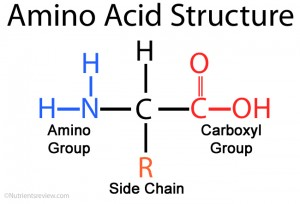
\includegraphics[scale=0.75]{images/AAS.jpg}
  \caption{Δομή ενός αμινοξέος}
  \label{fig:AAS}
\end{figure}


Η δευτεροταγής δομή των πρωτεΐνών αφορά τη γενικότερη 3-D αρχιτεκτονική των τοπικών στοιχείων της. Οι συνηθέστερες δευτερογενής δομές είναι:
\begin{enumerate}
    \item η "α-έλικα" δεξιόστροφη (a-helix) και
    \item η "β-πτυχωτή επιφάνεια" (b-sheets)
\end{enumerate}

\begin{figure}[h]
  \centering
  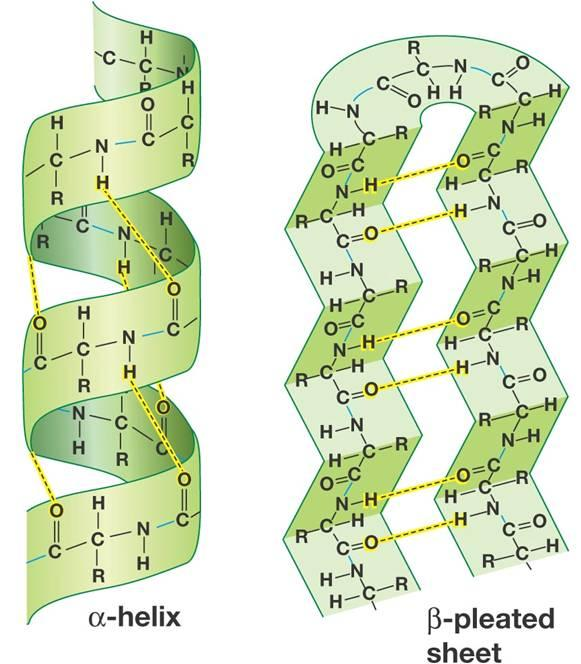
\includegraphics[scale=0.35]{images/sec_str.jpg}
  \caption{Δευτερογενής δομή πρωτεΐνών}
  \label{fig:sec_str}
\end{figure}
Όσον αφορά τις λειτουργίες των πρωτεϊνών, αυτές συναντώνται σε όλες τις διαστάσεις της κυτταρικής ζωής. Ορισμένες από αυτές παρουσιάζονται στον παρακάτω πίνακα:

\begingroup
\centering
\begin{tabularx}{1\textwidth} { 
  | >{\raggedright\arraybackslash}X 
  | >{\centering\arraybackslash}X 
  | >{\raggedleft\arraybackslash}X | }
  \hline
 \multicolumn{2}{|c|}{Λειτουργίες Πρωτεϊνών} \\
 \hline
 \textbf{Λειτουργία} & \textbf{Περιγραφή}\\
 \hline
 Άμυνα  & Πρωτεΐνες, όπως τα αντισώματα, δένονται πάνω σε άγνωστα σωματίδια (π.χ. ιοί, βακτήρια, προκειμένου να προστατεύσουν τον οργανισμό \\
\hline
Ένζυμο & Τα ένζυμα υλοποιούν σχεδόν όλες τις χημικές αντιδράσεις των κυττάρων. Ταυτόχρονα βοηθούν στη δημιουργία νέων μορίων διαβάζοντας τη γενετική πληροφορία που βρίσκεται αποθηκευμένη στο DNA.\\
\hline
Μεταφορά & Διάφορες πρωτεΐνες, όπως κάποια είδη ορμονών, μεταδίδουν σήματα για να συντονίσουν βιολογικές διεργασίες μεταξύ διαφορετικών κυττάρων, ιστών ή/και οργάνων. \\
\hline
Δομικό Στοιχείο & Παρέχουν δομή και στήριξη στα κύτταρα. Μακροσκοπικά, επιτρέπουν την κίνηση του οργανισμού. \\
\hline
Αποθήκευση & Δένουν και μεταφέρουν άτομα και μικρομόρια δια μέσω των κυττάρων σε όλο τον οργανισμο \\
\hline
\end{tabularx}
\captionof{table}{Λειτουργίες πρωτεϊνών}\label{Λειτουργίες πρωτεϊνών}
\endgroup


\section{Αλληλεπίδραση πρωτεΐνης με πρωτεΐνη}

Για να εκτελέσουν τις λειτουργίες τους μέσα στα κύτταρα, οι πρωτεΐνες σπανίως λειτουργούν ως απομονωμένες οντότητες. Αντιθέτως, πάνω από το 80\% των πρωτεϊνών εκτελούν τις λειτουργίες τους σε ομάδες\cite{Yanagida2002}, με την μέση πρωτεΐνη να αλληλεπιδρά με 3 εως 10 άλλες πρωτεΐνες\cite{Northey2017}. Μέσω της δημιουργίας ομάδων, οι πρωτεΐνες χειρίζονται ένα ευρύ φάσμα βιολογικών διεργασιών, μεταξύ των οποίων ο έλεγχος του μεταβολισμού και της ανάπτυξης των κυττάρων και η κυτταρική αλληλεπίδραση\cite{Rao2014}. Επομένως, ένα σημαντικό βήμα για την κατανόηση των μοριακών σχέσεων μεταξύ των οργανισμών είναι η "χαρτογράφηση" των φυσικών αλληλεπιδράσεων πρωτεΐνης με πρωτεΐνη (PPIs). 

\smallskip
Ως αλληλεπίδραση αναφερόμαστε στις συγκεκριμένες φυσικές επαφές μεταξύ ζεύγων πρωτεϊνών που συμβαίνουν μέσω επιλεκτικής μοριακής σύνδεσης σε ένα αυστηρά συγκεκριμένο βιολογικό πλαίσιο \cite{Rivas2010}. Η σύνδεση αυτή προκύπτει από μια πληθώρα βιοχημικών γεγονότων, μεταξύ των οποίων λόγω ηλεκτροστατικών δυνάμεων, δεσμών υδρογόνου και λόγω υδροφοβικότητας. Οι πρωτεΐνες συνδέονται μεταξύ τους μέσω περιοχών τους που είναι τόσο γεωμετρικά όσο και φυσιοχημικά συμπληρωματικές μεταξύ τους, οπότε και προκύπτουν ενεργειακά ευνοϊκές αλληλεπιδράσεις. Στον παρακάτω πίνακα παρουσιάζονται τα είδη των αλληλεπιδράσεων που αναπτύσσουν οι πρωτεΐνες μεταξύ τους:


\medskip
\begingroup
\begin{tabularx}{0.8\textwidth} { 
  | >{\raggedright\arraybackslash}X 
  | >{\centering\arraybackslash}X 
  | >{\raggedleft\arraybackslash}X | }
  \hline
 \multicolumn{3}{|c|}{Τύποι Αλληλεπιδράσεων Πρωτεΐνης με Πρωτεΐνη} \\
 \hline
    Με βάση την αλληλεπίδραση & Ομο-ολιγομερής (Homooligomeric) & Ετερο-ολιγομερής (Heterooligomeric)\\
 \hline
    Με βάση την ευστάθειά τους & Υποχρεωτικές (obligate) & Μη υποχρεωτικές (non obligate) \\
 \hline
    Με βάση το προσδόκιμο ζωής & Εφήμερες (Transient) & Σταθερές (Permanent) \\
 \hline
\end{tabularx}
\captionof{table}{Τύποι Αλληλεπιδράσεων Πρωτεΐνης με Πρωτεΐνη}\label{Τύποι Αλληλεπιδράσεων Πρωτεΐνης με Πρωτεΐνη}
\endgroup

\medskip
Ειδικότερα, \textit{oμοολιγομερείς} ονομάζονται οι αλληλεπιδράσεις μεταξύ ομοίων αλυσίδων ενώ \textit{ετεροολιγομέρεις} αυτές μεταξύ διαφορετικών αλυσίδων. Επιπλέον διαφοροποίηση παρατηρείται όσον αφορά την ευστάθεια των δεσμών,με τις αλληλεπιδράσεις να διακρίνονται σε \textit{υποχρεωτικές}, όπου τα πρωτομερή (δομικές μονάδες ολιγομερών πρωτεϊνών) δεν μπορούν να υπάρξουν ως ευσταθείς δομές \textit{in vivo}, και \textit{μη υποχρεωτικές}. Οι αλληλεπιδράσεις διαφοροποιούνται και όσον αφορά το προσδόκιμο ζωής της σύνδεσης. \textit{Σταθερές} ή \textit{μόνιμες} είναι αλληλεπιδράσεις με υψηλή ευστάθεια και μόνιμο χαρακτήρα, ενώ οι \textit{εφήμερες} αλληλεπιδράσεις αφορούν συνδέσεις και αποσυνδέσεις \textit{in vivo}. Ταυτόχρονα, υπάρχει ένας περαιτέρω διαχωρισμός των εφήμερων αλληλεπιδράσεων σε \textit{αδύναμες} (weak transient), όπου η ισορροπία συνεχώς χάνεται και ανακτάται, και \textit{ισχυρές} (strong transient),όπου απαιτείται κάποια μοριακή διατάραξη για να χαθεί η ισορροπία\cite{Nooren2003}. Αξίζει να σημειωθεί ότι οι περισσότερες PPIs δεν εντάσσονται σε κάποια διακριτή κατηγορία. Παραδείγματος χάριν, η ευστάθεια δεν αποτελεί μια συγκεκριμένη διαφοροποίηση αλλά ένα φάσμα όπου αλληλεπιδράσεις αλλάζουν ανάλογα με τις φυσιολογικές και περιβαλλοντικές συνθήκες.

\section{Μέθοδοι εντοπισμού αλληλεπιδράσεων πρωτεΐνης με πρωτεΐνη}

Η δημιουργία ομάδων πρωτεϊνών (\textit{protein complexes}) που προκύπτει από τις αλληλεπιδράσεις αυτών αυξάνει τον αριθμό των λειτουργικών στοιχείων και οδηγεί σε μεγαλύτερη ποικιλία πρωτεϊνών. Ωστόσο, ο πιθανός αριθμός συνδυασμών που μπορούν να δημιουργηθούν μέσω αλληλεπιδράσεων είναι τεράστιος, ενώ δεν είναι δυνατή η εξαγωγή γνώσης σχετικά με τη δημιουργία αυτών καθαρά από γονιδιωματική πληροφορία (\textit{genomic information}) \cite{Miura2018}.

\medskip
Παράλληλα, παρουσιάζονται δυσκολίες τόσο στην κατανόηση όσο και στην έρευνα των PPIs. Αυτό συμβαίνει διότι το αντικείμενο των PPIs είναι ένα διεπιστημονικό και εξειδικευμένο πεδίο που εκτείνεται από τη βιολογία (κατανόηση πρωτεϊνών) μέχρι τη φυσική (κινητικές ιδιότητες PPIs) και τη χημεία (χημικές ιδιότητες αλληλεπιδράσεων), με αποτέλεσμα μια εμπεριστατωμένη μελέτη να απαιτεί τη συνεργασία και την ενσωμάτωση γνώσης και μεθόδων των παραπάνω πεδίων. 

\subsection{Πειραματικές μέθοδοι εντοπισμού}

Οι πρώτες μέδοδοι εντοπισμού αφορούν την πειραματική έρευνα σχετικά με τους συνδυασμούς που μπορούν πραγματικά να δημιουργήσουν ομάδες, καθώς και τη μελέτη χαρακτηριστικών, όπως η χημική συγγένεια και οι κινητικές ιδιότητες των PPIs, προκειμένου να κατανοηθούν πλήρως οι πολύπλοκες βιολογικές διεργασίες στις οποίες συμμετέχουν.
Συνοπτικά, οι μέθοδοι πειραματικού εντοπισμού PPIs χωρίζονται σε 2 τύπους:

\begin{itemize}
    \item μέθοδοι \textit{in vitro}
    \item μέθοδοι \textit{in vivo} 
\end{itemize}

Κάθε μια από τις μεθόδους που παρουσιάζονται στη συνέχεια έχουν τα προτερήματά τους καθώς και τις αδυναμίες τους, ειδικά σε σχέση με την ευαισθησία (\textit{sensitivity}) και την εξειδίκευση (\textit{specificity}) τους.


\subsubsection{Μέθοδοι in vitro}

Στις μεθόδους \textit{in vitro}, μια συγκεκριμένη διαδικασία εκτελείται σε ένα ελεγχόμενο περιβάλλον εξωτερικά του ζωντανού οργανισμού. Οι συνηθέστερες in vitro μέθοδοι για τον εντοπισμό PPIs είναι οι tandem affinity purification, affinity chromatography, coimmunoprecipation,protein arrays, protein fragment complementation, phage display, X-ray crystallography and NMR spectroscopy.

\medskip
\textit{Tandem affinity purification}, γνωστή και ως μέθοδος \textit{TAP tagging}, είναι μια μέθοδος κάθαρσης βασιζόμενη στην ανοσοκαθίζηση, όπου ο σκοπός είναι η εξαγωγή από ένα κύτταρο μόνο μιας συγκεκριμένης πρωτεΐνης από όλες τις πρωτεΐνες με τις οποίες αλληλεπιδρούσε. Αναπτύχθηκε από τους Gavin et al. αρχικά για την ανάλυση των αλληλεπιδράσεων της μαγιάς \cite{Gavin2002}. Βασίζεται στον διπλό χαρακτηρισμό (tagging) της πρωτεΐνης ενδιαφέροντος σε επίπεδο χρωμοσωμάτων, ακολουθούμενο από μια διαδικασία κάθαρσης δυο βημάτων. Οι πρωτεΐνες που έπειτα από την κάθαρση παραμένουν συνδεδεμένες μπορούν στη συνέχεια να εντοπιστούν και να επεξεργαστουν (συνήθως ακολουθεί mass spectrometry (MS) επεξεργασία για τον υπολογισμό του λόγου μάζας προς φορτίο των ιόντων), με αποτέλεσμα τον εντοπισμό του βαθμού συμμετοχής της πρωτεΐνης ενδιαφέροντος στην αλληλεπίδραση. Η μεθοδος TAP tagging επιτρέπει την αναγνώριση μις πληθώρας αλληλεπιδράσεων ενώ επιτρέπει τον έλεγχο δραστηριότητας μονομερών και πολυμερών πρωτεϊνών in vivo.

\begin{figure}[h]
  \centering
  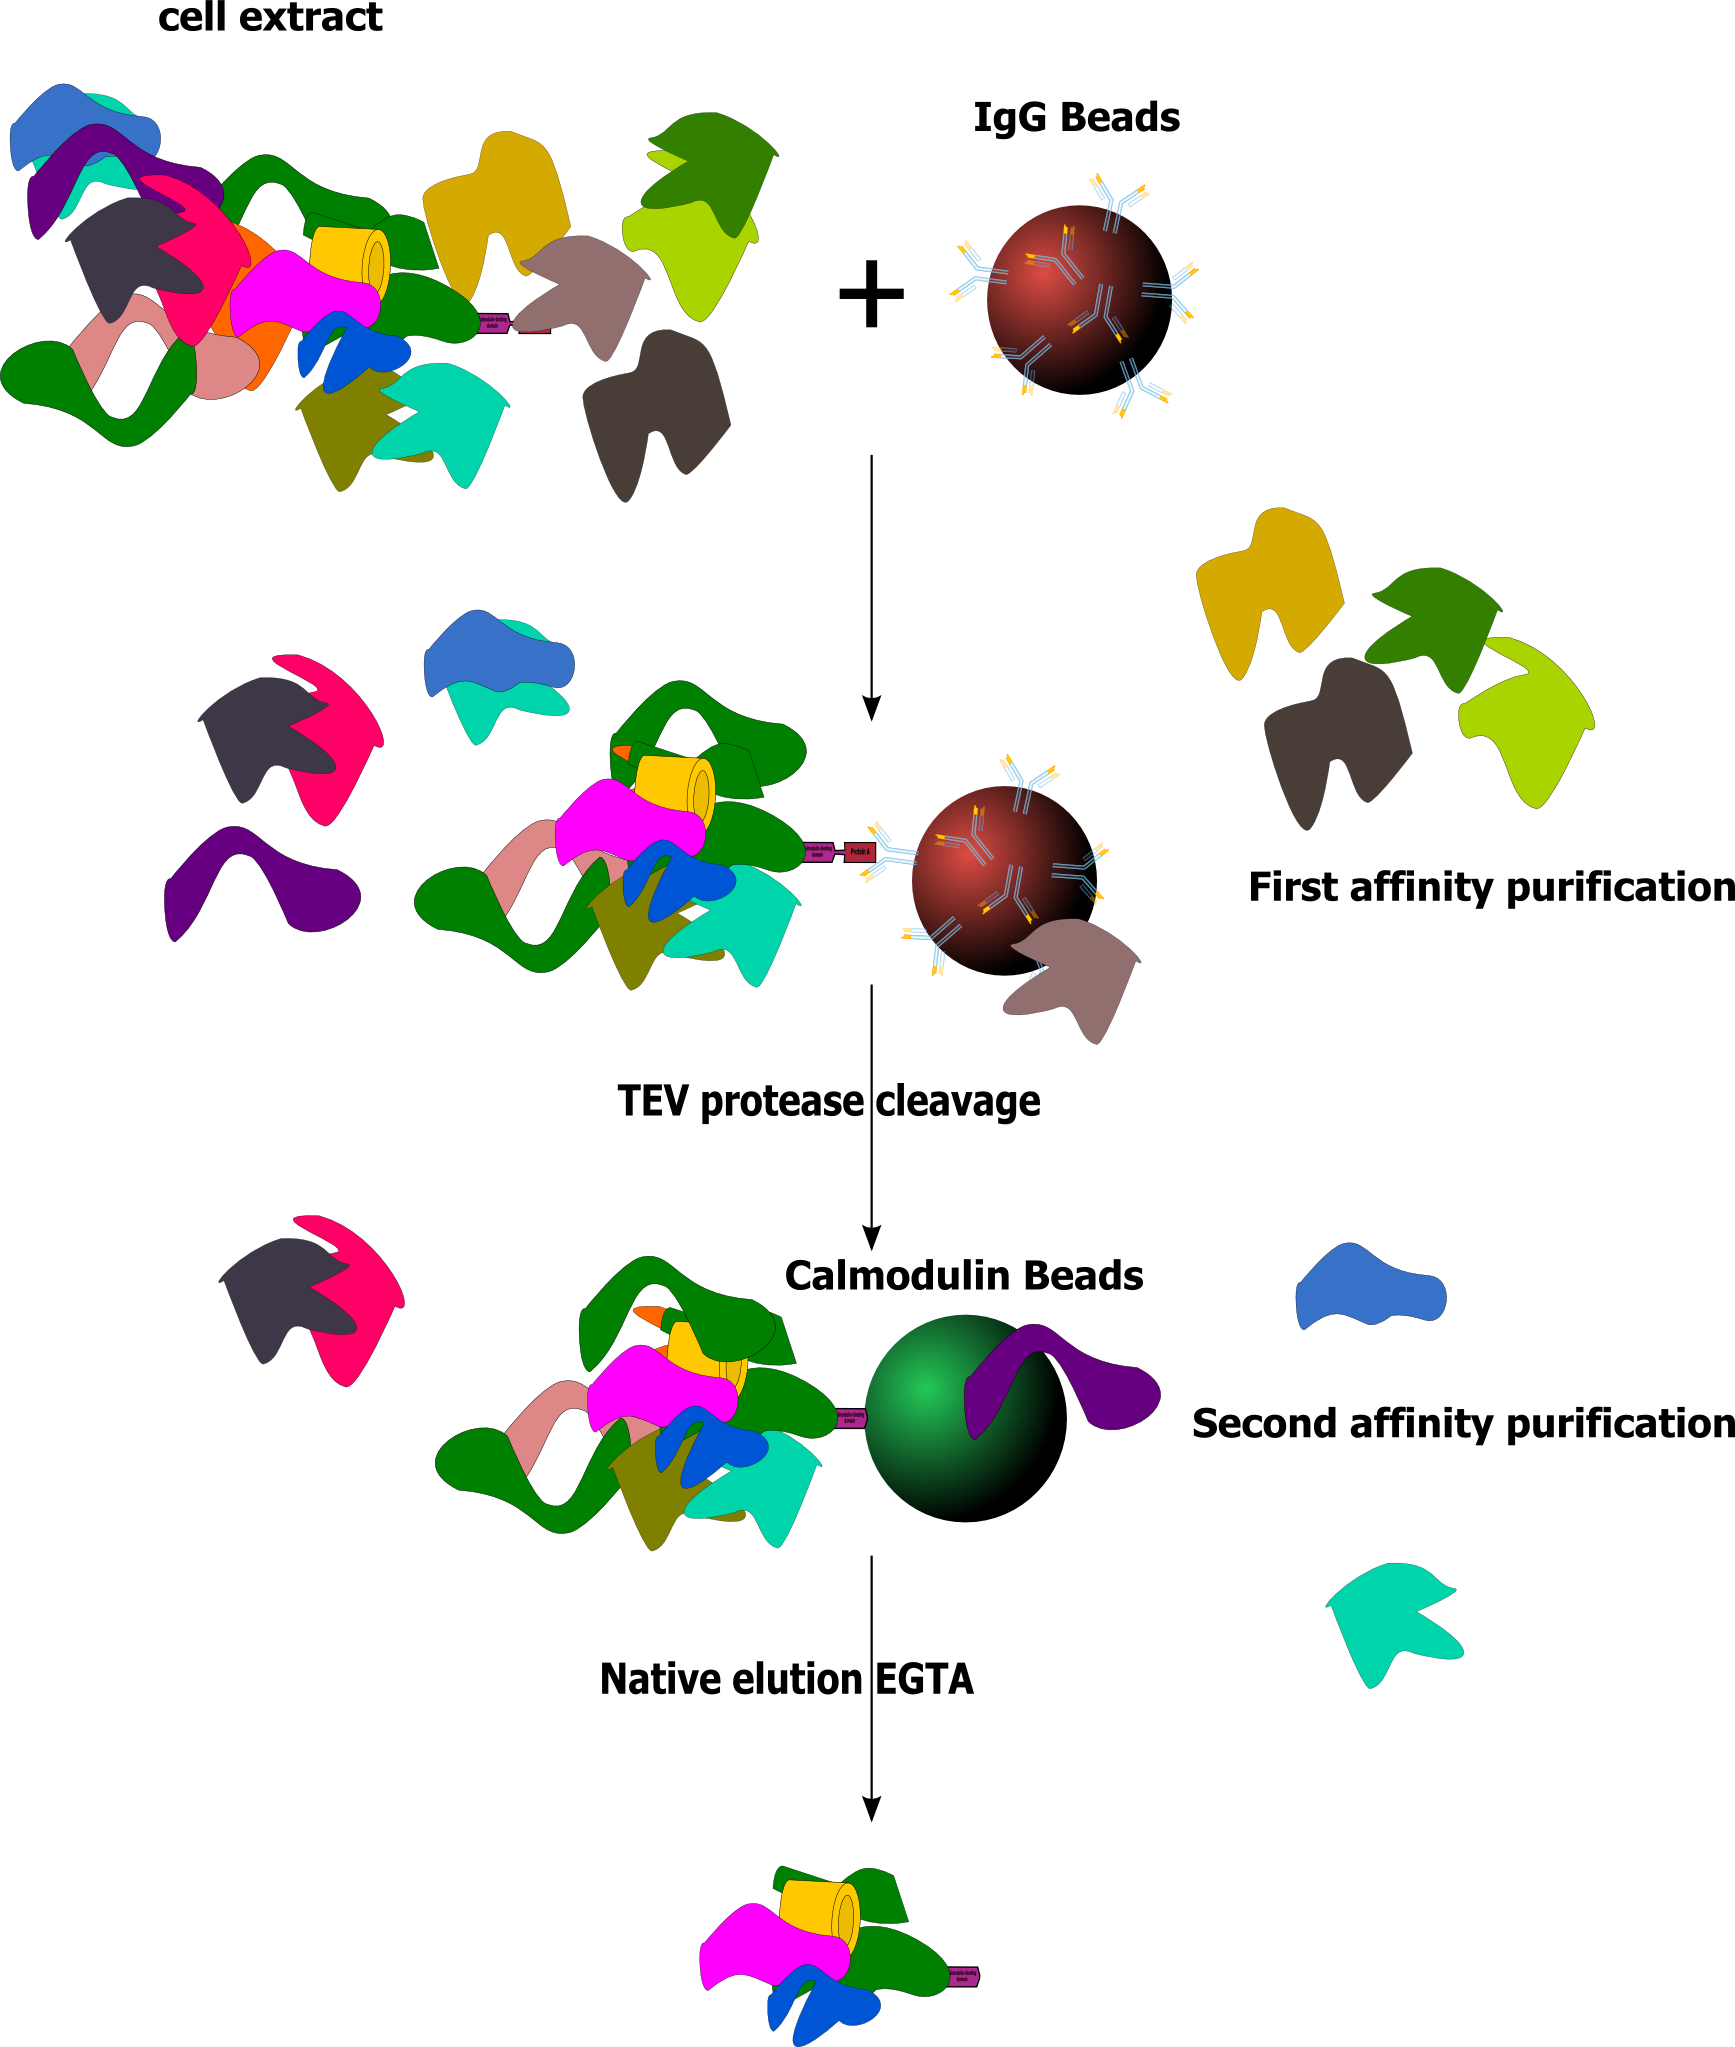
\includegraphics[scale=0.20]{images/Taptag_simple.png}
  \caption{Μέθοδος Tap Tagging}
  \label{fig:Taptag_simple}
\end{figure}

\textit{Affinity Chromatography}: Μια τεχνική επιλεκτικής κάθαρσης ενός μορίου ή μιας ομάδας μορίων από πολύπλοκες δομές βασισμένη σε εξαιρετικά συγκεκριμένες αλληλεπιδράσεις μεταξύ δυο μορίων\cite{Urh2009}. Ανήκει στις εργαστηριακές μεθόδους χρωματογραφίας και στα πλεονεκτήματά της παρουσιάζεται η γρήγορη αντιδρασιμότητα, η δυνατότητα εντοπισμού ακόμη και των ασθενέστερων αλληλεπιδράσεων ενώ ελέγχει ισόποσα κάθε πρωτεΐνη δείγματος όσον αφορά την αλληλεπίδραση της με την πρωτεΐνη ενδιαφέροντος. Ωστόσο, εμφανίζονται πολλές false positive αλληλεπιδράσεις που δεν υπάρχουν στο κυτταρικό σύστημα και αυτός ειναι ο κύριος λόγος που η εν λόγω τεχνική δεν μπορεί να χρησιμοποιηθεί εξ ολοκλήρου για τον έλεγχο και την αξιολόγηση PPIs. 

\textit{Co-immunoprecipation}: Είναι μια ευρέως διαδεδομένη μέθοδος για την αναγνώριση PPIs, ειδικά όταν εκτελείται σε ενδογενείς πρωτεΐνες. Αποτελεί μια επέκταση της ανοσοκαθίζησης, κατά την οποία με τη χρήση εξειδικευμένων για την πρωτεΐνη ενδιαφέροντος αντισωμάτων είναι δυνατή η απομόνωση της συγκεκριμένης πρωτεΐνης, καθώς και άλλων μακρομορίων που παραμένουν μετά την αντίδραση συνδεδεμένα με αυτήν, από τον υπόλοιπο κυτταρικό ιστό\cite{Golemis2002}. Η διαφορά με τις immunoprecipation μεθόδους βρίσκεται στο αντικείμενο του πειράματος, που δεν ειναι πλεον η μελέτη της πρωτεΐνης ενδιαφέροντος αλλα η μελέτη των μακρομορίων με τα οποία αλληλεπιδρά.

\begin{figure}[h]
  \centering
  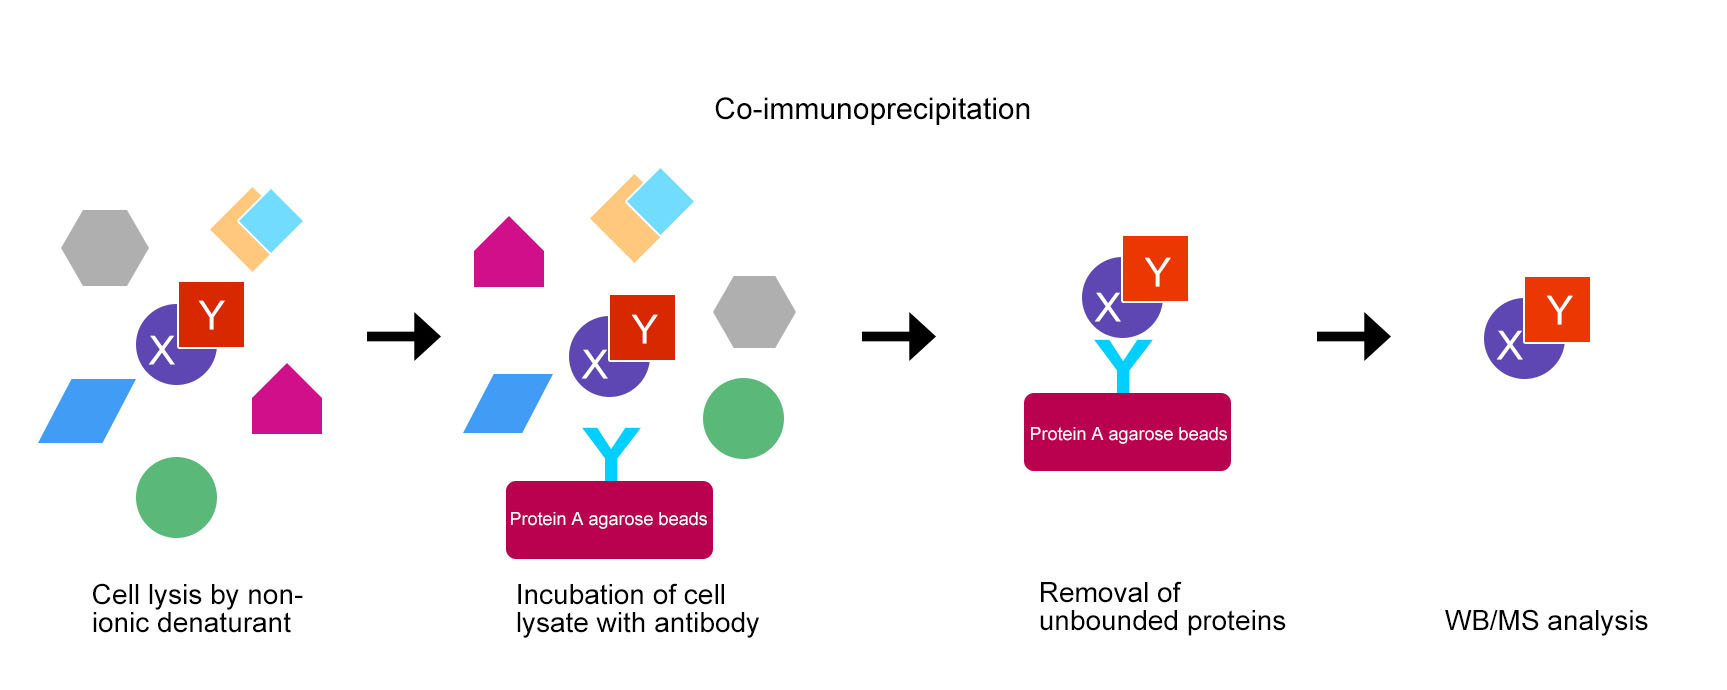
\includegraphics[scale=0.22]{images/Coip.jpg}
  \caption{Μέθοδος Co-immunoprecipation}
  \label{fig:coip}
\end{figure}

Οι \textit{μικροσυστοιχίες πρωτεϊνών} (protein microarrays) αποτελούν μια απο τις πιο εξελισσόμενες τεχνικές όσον αφορά τον εντοπισμό πρωτεϊνών, καθώς και την διερεύνηση των λειτουργιών και των αλληλεπιδράσεών τους. Μια μικροσυστοιχία πρωτεϊνών είναι ένα κομμάτι γυαλί, πάνω στο οποίο τοποθετούνται μόρια πρωτεϊνών σε ορισμένες αποστάσεις μεταξύ τους\cite{MacBeath2000}. Τα πλεονεκτήματα τους βρίσκονται στην δυνατότητα παράλληλης και αυτοματοποιημένης ανάλυσης πολλαπλών μικροσυστοιχιών με μεγάλη ακρίβεια.


\textit{Protein-fragment complementation assays}: Aποτελούν μια οικογένεια πειραμάτων για τον εντοπισμό PPIs. Στα PCAs, οι πρωτεϊνες αλληλεπίδρασης (οπου ονομάζονται δόλωμα-bait και λεία-prey) συνδέονται μέσω ομοιοπολικών δεσμών με μια τρίτη πρωτεΐνη, που δρα ως reporter. Οι αλληλεπιδράσεις μεταξύ των πρωτεϊνών ενδιαφέροντος φέρνουν τα αντίστοιχα μέρη της πρωτεΐνης reporter κοντά, προκειμένου να δημιουργηθεί μια λειτουργική πρωτεΐνη reporter, η οποία μπορεί να μετρηθεί. Μέσω των PCAs μπορούν να εντοπιστούν PPIs μεταξύ πρωτεϊνών ανεξαρτήτως βάρου σε ενδογενές επίπεδο\cite{Michnick2011}.

\begin{figure}[h]
  \centering
  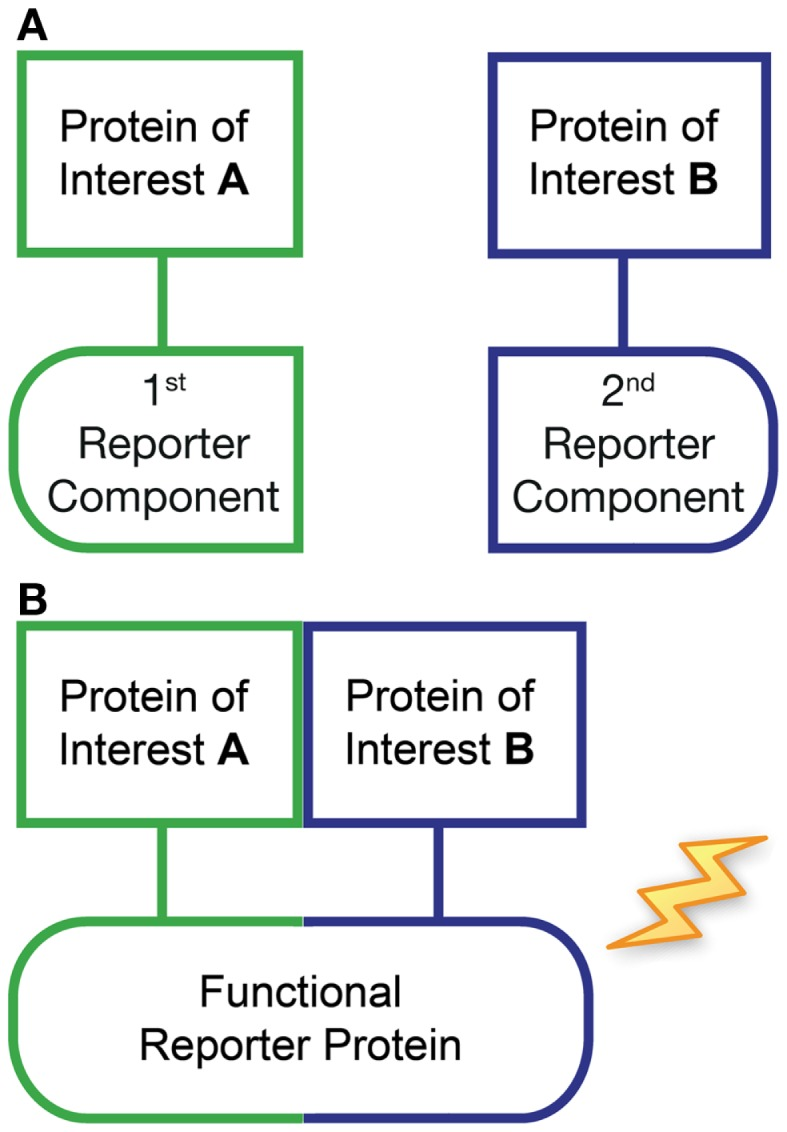
\includegraphics[scale=0.20]{images/PCA.png}
  \caption{Απλοποιημένη αναπαράσταση PCAs}
  \label{fig:PCA}
\end{figure}

\newpage
\textit{Phage Display}: Αποτελεί μια εργαστηριακή μέθοδο για την μελέτη των PPIs που κάνει χρήση βακτηριοφάγων ( αλλιώς φάγων, δηλαδή ιων που μολύνουν βακτήρια) για να συνδέσουν πρωτεΐνες μεσω της γενετική πληροφορία που τις κωδικοποιεί \cite{Smith1985}. Η διαδικασία περιλαμβάνει την εισαγωγή γενετικής πληροφορίας μιας πρωτεΐνης ενδιαφέροντος σε έναν φάγο, με αποτέλεσμα να "προβάλλεται" η πρωτεΐνη στο εξωτερικό του φάγου ενώ η γενετική πληροφορία να παραμένει στο εσωτερικό του. Αυτοι οι φάγοι, που ονομάζονται και \textit{display phages}, προβάλλονται πάνω σε άλλες πρωτεΐνες προκειμένου να εντοπιστούν πιθανές αλληλεπιδράσεις.

\begin{figure}[h]
  \centering
  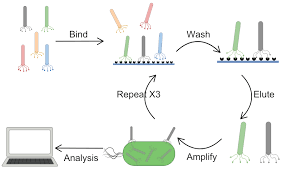
\includegraphics[scale=0.8]{images/phagedisplay.png}
  \caption{Κύκλος μεθόδου Phage Display}
  \label{fig:phagedisplay}
\end{figure}

H κρυσταλλογραφία με ακτίνες Χ (\textit{X-ray crystallography}) είναι μια μορφή μικροσκοπίας υψηλής ευκρίνειας, με σκοπό την οπτικοποίηση της ατομικής και μοριακής δομής των πρωτεϊνών, επιτρέποντας περαιτέρω κατανόηση των λειτουργιών τους. Βασίζεται στη διάθλαση ακτίνων Χ, ύστερα απο πρόσκρουσή τους στην κρυσταλλική δομή των πρωτεϊνών, προς συγκεκριμένες κατεθύνσεις. Με την τεχνική αυτή είναι δυνατός ο σχεδιασμός καινοτόμων φαρμάκων που στοχεύουν συγκεκριμένες πρωτεΐνες \cite{Tong2001}.

Τέλος, τα τελευταία χρόνια παρουσιάζεται έντονο ερευνητικό ενδιαφέρον στην ανάλυση PPIs μέσω \textit{nuclear magnetic resonance spectroscopy} (NMR). Η βάση της NMR spectroscopy είναι ότι οι μαγνητικά ενεργοί κυτταρικοί πυρήνες, όταν προσανατολίσονται υπό ένα ισχυρό μαγνητικό πεδίο, απορροφούν ηλεκτρομαγνητικη ακτινοβολία σε χαρακτηριστικές συχνότητες που εξαρτώνται απο το χημικό τους περιβάλλον. Εξετάζοντας τα διαφορετικά επίπεδα απορρόφησης ακτινοβολίας, οι ερευνητές μπορούν να αποκτήσουν εικόνα για την ηλεκτρονιακή δομή των μορίων και την λειτουργία τους \cite{OConnell2009}.


\subsubsection{Μέθοδοι in vivo}

Στις μεθόδους \textit{in vivo}, μια συγκεκριμένη διαδικασία εκτελείται σε ελεγχόμενο περιβάλλον εντός του ζωντανού οργανισμου. Οι μέθοδοι in vivo για τον εντοπισμό PPIs είναι: yeast two-hybrid (Y2H, Y3H) και synthetic lethality.

\textit{Yeast two-hybrid} ή two-hybrid screening είναι μια τεχνική μοριακής βιολογίας που χρησιμοποιείται για τον εντοπισμό PPIs ερευνώντας για πιθανές φυσικές αλληλεπιδράσεις μεταξύ είτε δύο πρωτεϊνών που αναμένουμε να αλληλεπιδρούν είτε βρίσκοντας πρωτεΐνες (prey) που αλληλεπιδρούν με μια συγκεκριμένη πρωτεΐνη (bait) \cite{Uetz2000}. Αποτελεί μια in vivo τεχνική protein-fragment complementation, οικογένεια πειραμάτων που αναφέρθηκε στις in vitro τεχνικές. Ειδικότερα, το πείραμα εκτελείται εισάγοντας δύο πρωτεϊνες ενδιαφέροντος σε μαγιά, με κάθε πρωτεϊνη να ενώνεται με έναν \textit{transcription factor - TF} που έχει χωριστεί σε δυο πανομοιότυπα κομμάτια. Πρωτεϊνες που αλληλεπιδρούν μεταξύ τους οδηγούν στη δημιουργία ενός λειτουργικού TF όταν έρθουν σε κοντινή απόσταση. Παρ' ότι ιδιαίτερα χρήσιμη τεχνική, οδηγεί στη δημιουργία πολλών false positive αλληλεπιδράσεων, ενώ το τελικό σύνολο PPIs είναι μικρό σε αριθμό, καθώς εισάγουν έναν μεγάλο παράγοντα false negative αλληλεπιδράσεων. Τέλος, επειδή χρησιμοποιεί τη μαγιά ως host, δημιουργεί προβλήματα κατά τη μελέτη πρωτεϊνών που περιέχουν συγκεκριμένες για τα θηλαστικά τροποποιήσεις \cite{Schneider2016}. 

Synthetic lethality: Πρόκειται για μια in vivo γενετική τεχνική που προσπαθεί να κατανοήσει τους μηχανισμούς που επιτρέπουν φαινοτυπική ισορροπία σε ένα κύταρρο/ οργανισμό παρά τις αλλαγές σε γενετικό και περιβαλλοντικό επίπεδο. Η έννοια synthetic lethality προκύπτει όταν η ταυτόχρονη διαταραχή δυο γονιδίων οδηγεί σε κυτταρικό θάνατο ή στον θάνατο του οργανισμού, ενώ η διαταραχή μονάχα ενός εκ των δυο γονιδίων δεν έχει τέτοια αποτελέσματα. Συνεπώς, η τεχνική αυτή προσπαθεί να δημιουργήσει μεταλλάξεις σε γονίδια που είναι βιώσιμα μόνα τους αλλά προκαλούν τοξικότητα σε συνδυασμό μεταξύ τους ύπο συγκεκριμένες συνθήκες \cite{Ooi2006}. Ωστόσο, αξίζει να αναφερθεί ότι οι σχέσεις που εντοπίζονται από την τεχνική synthetic lethality δεν απαιτούν φυσικές αλληλεπιδράσεις μεταξύ των πρωτεϊνών ενδιαφέροντος, με αποτέλεσμα να αποκαλούμε αυτού του είδους τις αλληλεπιδράσεις ως \textit{λειτουργικές αλληλεπιδράσεις (functional interractions)}.

\begin{figure}[h]
  \centering
  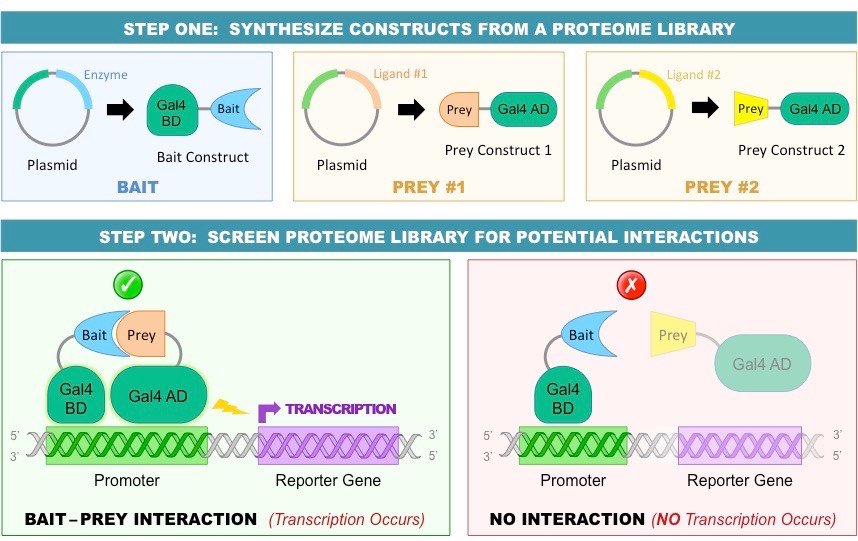
\includegraphics[scale=0.4]{images/yeast-2-hybrid_med.jpeg}
  \caption{Μέθοδος Yeast Two-Hybrid}
  \label{fig:yeast-2-hybrid_med}
\end{figure}

\begin{figure}[h]
  \centering
  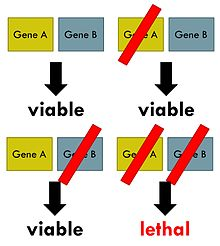
\includegraphics[scale=0.75]{images/Synthetic_lethality.jpg}
  \caption{Παράδειγμα Synthetic Lethality}
  \label{fig:Synthetic_lethality}
\end{figure}

\newpage
\begingroup
\centering
\begin{tabularx}{0.9\textwidth} { 
  | >{\raggedright\arraybackslash}X 
  | >{\centering\arraybackslash}X 
  | >{\raggedleft\arraybackslash}X | }
 \hline
 \textbf{Τεχνική} & \textbf{Περιγραφή}\\
 \hline
 Tandem affinity purification (TAP) & Βασίζεται στον διπλό χαρακτηρισμό μιας πρωτεΐνης σε επίπεδο χρωμοσωμάτων.\\
 \hline
 Affinity Chromatography & Τεχνική επιλεκτικής κάθαρσης ενός μορίου ή μιας ομάδας μορίων από πολύπλοκες δομές βασισμένη σε εξαιρετικά συγκεκριμένες αλληλεπιδράσεις μεταξύ δυο μορίων.\\
 \hline
 Co-immunoprecipation & Επιβεβαιώνει αλληλεπιδράσεις με τη χρήση με τη χρήση εξειδικευμένων για την πρωτεΐνη ενδιαφέροντος αντισωμάτων.\\
 \hline
 Protein Microarrays & Ανάλυση βασισμένη σε μικροσυστοιχίες που επιτρέπει την ταυτόχρονη επεξεργασία χιλλιάδων παραμέτρων μέσα σε ένα μόνο πείραμα.\\
 \hline
 Protein-fragment complementation assays & Χρηση για τον εντοπισμό PPIs μεταξύ πρωτεϊνών ανεξαρτήτως μεγέθους και εκφρασμένες σε ενδογενές επίπεδο.\\
 \hline
 Phage Display & Στηρίζεται στην ενσωμάτωση της δομικής και γενετικής πληροφορίας μιας πρωτεϊνης σε έναν βακτηριοφάγο.\\
 \hline
 X-ray crystallography & Οπτικοποίηση υψηλής ευκρίνειας μέσω κρυσταλλογραφίας με ακτίνες Χ.\\
 \hline
 NMR spectroscopy & Εντοπισμός PPIs μέσω απορρόφησης ηλεκτρομαγνητικής ακτινοβολίας των πυρήνων των πρωτεϊνών.\\
 \hline
\end{tabularx}
\captionof{table}{Σύνοψη in vitro τεχνικων εντοπισμού PPIs} 
\label{In vitro τεχνικές εντοπισμού PPIs}
\endgroup

\begingroup
\centering
\begin{tabularx}{1\textwidth} { 
  | >{\raggedright\arraybackslash}X 
  | >{\centering\arraybackslash}X 
  | >{\raggedleft\arraybackslash}X | }
 \hline
 \textbf{Τεχνική} & \textbf{Περιγραφή}\\
 \hline
 Yeast two-hybrid (Y2H) & Τεχνική που εκτελείται αξιολογώντας μια πρωτεΐνη ενδιαφέροντος πάνω σε μια τυχαία βιβλιοθήκη από πιθανές πρωτεΐνες αλληλεπίδρασης. \\ 
 \hline
 Synthetic lethality & Γενετική τεχνική που αξιολογεί τις λειτουργικές αλληλεπιδράσεις (και όχι τις φυσικές αλληλεπιδράσεις). \\
 \hline
 \end{tabularx}
 \captionof{table}{Σύνοψη in vivo τεχνικώ εντοπισμού PPIs} 
\label{In vivo τεχνικές εντοπισμού PPIs}
 \endgroup
 
 

\subsection{Υπολογιστικές μέθοδοι εντοπισμού}

Η μέθοδος yeast two-hybrid, καθώς και πολλές άλλες \textit{in vitro} και \textit{in vivo} μέθοδοι, οδήγησαν στην ανάπτυξη μιας μεγάλης γκάμας από χρήσιμα εργαλεία για τον εντοπισμό PPIs μεταξύ ορισμένων πρωτεϊνών που μπορούν να αλληλεπιδράσουν με πολλαπλούς συνδυασμούς. Παρ' όλα αυτά, τα αποτελέσματα των παραπάνω μεθόδων μπορεί να μην είναι αξιόπιστα λόγω της περιορισμένης γνώσης γύρω από τις πιθανές PPIs. Για την πλήρη κατανόηση των πιθανών αλληλεπιδράσεων, κρίθηκε σκόπιμη η δημιουργία προσεγγίσεων που προβλέπουν όλες τις πιθανές αλληλεπιδράσεις μεταξύ πρωτεϊνών \cite{Zhang2009}.

Μια πληθώρα από μεθόδους \textit{in silico}, δηλαδή εκτελεσμένες σε υπολογιστή ή μέσω υπολογιστικής προσωμοίωσης, αναπτύχθηκαν για να στηρίξουν τις αλληλεπιδράσεις που προέκυψαν μέσω των παραπάνω πειραματικών μεθόδων. Ορισμένες από τις υπολογιστικές μεθόδους που έχουν αναπτυχθεί είναι:
structure-based approaches,sequence-based approaches, εγγύτητα χρωμοσωμάτων (chromosome proximity), gene fusion, in silico 2 hybrid, mirror tree, phylogenetic profiling και gene expression-based approaches.

\medskip
\textit{Structure-based approaches}: Η βασική ιδέα που διέπει τις μεθόδους εντοπισμού PPIs μέσω δομικών προσεγγίσεων είναι η πρόβλεψη αλληλεπιδράσεων εαν δύο πρωτεΐνες έχουν παρόμοια δομή. Για παράδειγμα, ένας πρόσφατος αλγόριθμος για structure-based prediction of PPIs, ο \textbf{Coev2Net}, ακολουθεί μια διαδικασία τριων βημάτων, που χωρίζεται σε:

\begin{itemize}
    \item πρόβλεψη της επιφάνειας αλληλεπίδρασης,
    \item αξιολόγηση της συμβατότητας της επιφάνειας για αλληλεπίδραση μέσω ενός βασικού μοντέλου \textit{coevolution} και
    \item αξιολόγηση του confidence score της αλληλεπίδρασης \cite{Hosur2011}.
\end{itemize}

\newpage
\textit{Sequence-based approaches}: Οι προβλέψεις για PPIs βασίζονται στην ενσωμάτωση γνώσης γνωστών PPIs με τη γνώση που αφορά την ακολουθιακή ομολογία. Με άλλα λόγια, μια αλληλεπίδραση που εντοπίζεται σε ένα είδος μπορεί να χρησιμοποιηθεί ως βάση για τον εντοπισμό της ίδιας αλληλεπίδρασης σε άλλα είδη. Οι sequence-based approaches χωρίζονται σε δύο διακριτές κατηγορίες:
\begin{enumerate}
    \item Ortholog-Based προσεγγίσεις και
    \item Domain-Pairs-Based προσεγγίσεις.
\end{enumerate}

\smallskip
1. \textit{Ortholog-Based} προσέγγιση: Στηρίζεται στην μεταφορά παρατηρήσεων από μια λειτουργικά ορισμένη πρωτεϊνική ακολουθία στην πρωτεϊνική ακολουθία ενδιαφέροντος, βασισμένοι στην ομοιότητά τους. Η παρατήρηση μέσω ομοιότητας προκύπτει με την χρήση αλγορίθμων τοπικής αναζήτησης ανα ζεύγη και στηρίζεται στο βαθμό ομοιότητας της πρωτεΐνης ενδιαφέροντος με πρωτεΐνες σε μια βάση δεδομένων πρωτεϊνών \cite{Lee2008}. Η προσέγγιση ονομάζεται ortholog-based καθώς στηρίζεται στην έννοια της ορθολογικότητας, δηλαδή της ανάπτυξης γονιδίων σε διαφορετικά είδη που προέρχονται από ένα κοινό προγονικό γονίδιο μέσω συσχέτισης.

\smallskip
2. \textit{Domain-Pairs-Based} προσέγγιση: Η προσέγγιση αυτή αφορά τα domains, που αποτελούν ένα διακριτό,συμπαγές και ευσταθές μέρος της πρωτεϊνικής ακολουθίας (συγκεκριμένα της τεταρτοταγούς δομής των πρωτεϊνών) που μπορεί να εξελιχθεί, να λειτουργήσει και να υπάρξει ανεξάρτητα από την υπόλοιποη πρωτεϊνική αλυσίδα. Ως ατομικά δομικά και λειτουργικά μέρη μιας πρωτεΐνης, τα protein domains παίζουν σημαντικό ρόλο στην ανάπτηξη της πρόβλεψης πρωτεϊνικών δομικών κλάσεων, στην προβλεψη τύπων πρωτεϊνικών μεμβρανών, στην πρόβλεψη ενζυμικής κλάσης κ.α. Θεωρούνται θεμελιώδη για την αλληλεπίδραση πρωτεϊνών καθώς είναι άμεσα συνδεδεμένα με την διαμοριακή αλληλεπίδραση, επομένως είναι αρκετά αξιόπιστη η χρήση των domains και των αλληλεπιδράσεών τους για την πρόβλεψη PPIs και αντίστροφα \cite{Wojcik2001}.

\begin{figure}[h]
  \centering
  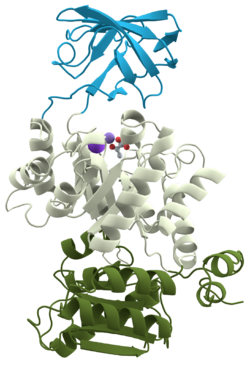
\includegraphics[scale=0.48]{images/Pyruvate_kinase_protein_domains.png}
  \caption{Παράδειγμα πρωτεΐνη με 3 domains (\textit{Pyruvate kinase})}
  \label{fig:Pyruvate_kinase_protein_domains}
\end{figure}

\smallskip
\textit{Chromosome Proximity}: Είναι γνωστό ότι λειτουργικά παρόμοιες πρωτεΐνες τείνουν να οργανώνονται πολύ κοντά σε περιοχές στα γονιδιώματα των προκαρυωτικών οργανισμών. Συνεπώς, δημιουργήθηκε η ιδέα πως αν αυτή η σχέση γειτνίασης των πρωτεϊνών παρατηρηθεί σε πολλαπλά γονιδιώματα, τότε μπορεί να υπάρχει πιθανή λειτουργική σύνδεση μεταξύ των πρωτεϊνών στα αντίστοιχα γονιδιώματα. Η ιδέα αυτή επιβεβαιώθηκε πειραματικά \cite{Yamada2003} και χρησιμοποιήθηκε για τη μελέτη της λειτουργικής σχέσης των πρωτεϊνών, καθώς και την πρόβλεψη αλληλεπιδράσεων.

\smallskip
\textit{Gene Fusion}: Γνωστή και ως \textit{Rosetta stone method}, βασίζεται στην τάση ορισμένων πρωτεϊνών που περιέχουν ένα μόνο domain σε έναν οργανισμό να συγχωνεύονται για να δημιουργήσουν multidomain πρωτεΐνες σε άλλους οργανισμους \cite{Enright1999}. Το άνοθεν φαινόμενο πρωτεϊνικής συγχώνευσης υποννοεί την πιθανή λειτουργική αλληλεπίδραση των ξεχωριστών πρωτεϊνών. Με τη χρήση πληροφορίας σχετικά με τη διάταξη των domains σε διαφορετικά γονιδιώματα, γίνεται πρόβλεψη πρωτεϊνικών αλληλεπιδράσεων \cite{Marcotte1999}. Ωστόσο, μπορεί να εφαρμοστεί μόνο σε πρωτεΐνες όπου έχουν παρατηρηθεί οι συγκεκριμένες διατάξεις των domains.

\smallskip
\textit{In Silico Two-Hybrid}: Θεωρία που βασίζεται στον ισχυρισμό ότι οι πρωτεΐνες που αλληλεπιδρούν θα πρέπει να υφίστανται ταυτόχρονη εξέλιξη (\textit{co-evolution}) προκειμένου να διατηρήσουν τις λειτουργίες τους αξιόπιστες. Με άλλα λόγια, αν ορισμένα αμινοξέα της μιας πρωτεΐνης υποστούν κάποια αλλαγή, τότε τα αντίστοιχα αμινοξέα της άλλης πρωτεΐνης θα πρέπει να υποστούν τις αναγκαίες μεταλλάξεις, προκειμένου η σύνδεση να παραμείνει λειτουργική. Καθώς η συγκεκριμένη ανάλυση στηρίζεται στην πρόβλεψη της φυσικής εγκύτητας μεταξύ ζευγαριών residues ανάμεσα σε δυο πρωτεΐνες, αυτόματα τα αποτελέσματα υποδεικνύου και πιθανές φυσικές αλληλεπιδράσεις \cite{Pazos2002}.

\smallskip
\textit{Phylogenetic Tree - Mirror Tree Method}: Μια ακόμη υπολογιστική μέθοδος που χρησιμοποείται για τον εντοπισμό PPIs είναι το \textit{φυλογενετικό δέντρο}. Το \textit{φυλογενετικό δέντρο} παρέχει την πληροφορία της εξέλιξης μιας πρωτεΐνης. Σε αυτό βασίζεται η μέθοδος \textit{mirror tree}, όπου υποστηρίζεται ότι οι πρωτεΐνες που αλληλεπιδρούν μεταξύ τους θα παρουσιάζουν παρόμοια φυλογενετικά δέντρα, λόγω του παράγοντα co-evolution που υπάρχει καθ' όλη την αλληλεπίδραση \cite{Sato2005}. Ειδικότερα, η βασική αρχή πίσω από την θεωρία είναι ότι ο παράγοντας co-evolution αντανακλάται στο βαθμό ομοιότητας που παρουσιάζουν οι πίνακες απόστασης των φυλογενετικών δέντρων των αλληλεπιδρόντων πρωτεϊνών \cite{Craig2007}. Υψηλοί βαθμοί συσχέτισης υποδεικνύουν την σχέση co-evolution των πρωτεϊνών και με τη χρήση αυτής της σχέσης εξάγονται συμπεράσματα για την πιθανότητα φυσικής αλληλεπίδρασης μεταξύ αυτών.

\begin{figure}[h]
  \centering
  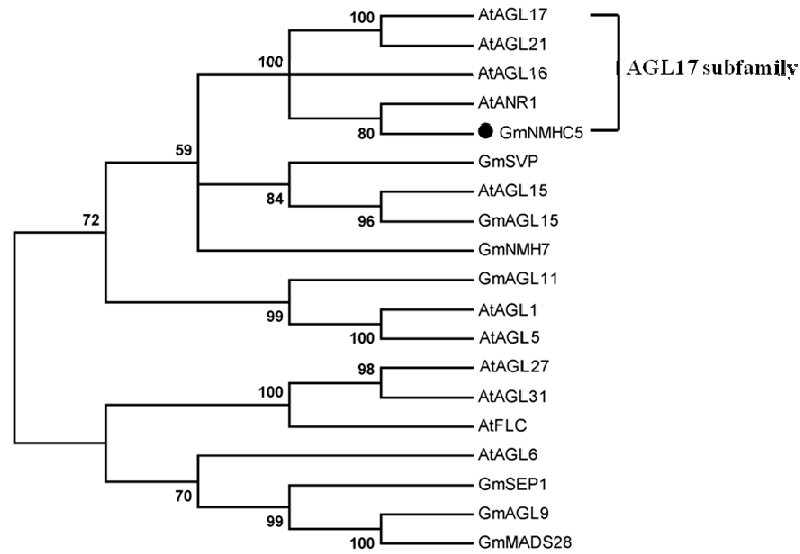
\includegraphics[scale=1]{images/Phylogenetic-tree.png}
  \caption{Παράδειγμα φυλογενετικού δέντρου}
  \label{fig:Phylogenetic-tree}
\end{figure}

\smallskip
\textit{Phylogenetic Profile}: Στηρίζεται στην θεωρία ότι λειτουργικά συνδεδεμένες πρωτεΐνες τείνουν να συνυπάρχουν κατά την εξέλιξη ενος οργανισμού. Με άλλα λόγια, αν δυο πρωτεΐνες έχουν μια λειτουργική σύνδεση σε ένα γονιδίωμα, θα υπάρχει ισχυρή "πίεση" ώστε να υιοθετηθούν μαζί κατά τη διαδικασία της εξέλιξης  \cite{Srinivas2008}. Επομένως, τα ορθόλογα τους σε άλλα γονιδιώματα είτε θα έχουν διατηρηθεί είτε θα έχουν απορριφθεί (η έννοια της ορθολογικότητας παρουσιάστηκε στη σελίδα 15 - Ortholog-Based προσέγγιση). Για τον εντοπισμό της ύπαρξης ή όχι των πρωτεϊνών αυτών χρησιμοποιείται το \textit{φυλογενετικό προφίλ}, που περιγράφει την εμφάνιση μιας πρωτεΐνης σε ένα σετ γονιδιωμάτων. Συνεπώς, αν δύο πρωτεΐνες μοιράζονται το ίδιο φυλογενετικό προφίλ, τότε είναι αρκετά πιθανή η λειτουργική τους σύνδεση. Όμως, παρ' ότι η μέθοδος έχει υποσχόμενα αποτελέσματα στον εντοπισμό PPIs, βασίζεται σε ολοκληρωμένες ακολουθίες γονιδιωμάτων (γεγονός που περιορίζει την γενίκευση της μεθόδου) ενώ παράλληλα διάφορα γεγονότα κατά την διαδικασία του co-evolution, οπως η αντιγραφή γονιδιωμάτων ή η απώλεια λειτουργιών, μπορούν να διαφθείρουν το φυλογενετικό προφιλ, επηρεάζοντας την απόδοση της μεθόδου \cite{Lin2013}.

\begin{figure}[h]
  \centering
  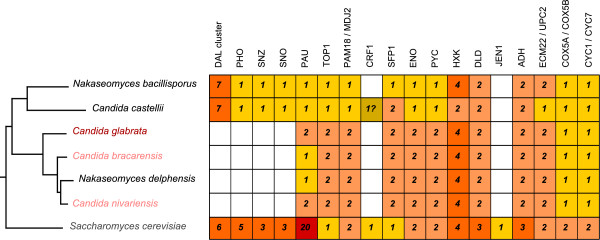
\includegraphics[scale=0.6]{images/Phylogenetic-profile.png}
  \caption{Παράδειγμα φυλογενετικού προφίλ}
  \label{fig:Phylogenetic-profile}
\end{figure}


\textit{Gene Expression}: Η έννοια gene expression σημαίνει την ποσοτικοποίηση του επιπέδου στο οποίο ένα συγκεκριμένο γονίδιο εκφράζεται μέσα σε ένα κύτταρο/ιστό/οργανισμό κάτω από διαφορετικές περιβαλλοντικές και χρονικές συνθήκες. Μέσω της εφαρμογής αλγορίθμων συσταδοποίησης, γίνεται ομαδοποίηση γονιδίων ανάλογα με τον βαθμό έκφρασής τους, επομένως το αποτέλεσμα μπορεί να βοηθήσει στη διατύπωση των λειτουργικών σχέσεων των ομαδοποιημένων γονιδίων, καθώς πρωτεΐνες από γονίδια που ανήκουν στην ίδια συστάδα έχουν μεγαλύτερη πιθανότητα αλληλεπίδρασης μεταξύ τους απότι με πρωτεΐνες από άλλες συστάδες \cite{Grigoriev2001}.

\medskip
\begingroup
\centering
\begin{tabularx}{0.9\textwidth} { 
  | >{\raggedright\arraybackslash}X 
  | >{\centering\arraybackslash}X 
  | >{\raggedleft\arraybackslash}X | }
 \hline
 \textbf{Τεχνική} & \textbf{Περιγραφή}\\
 \hline
 Structure-based approach & Πρόβλεψη PPIs εαν δύο πρωτεΐνες έχουν παρόμοια δομή (πρωτοταγή, δευτεροταγή ή τεταρτοταγή). \\ 
 \hline
 Ortholog-based approach & Sequence-based τεχνική βασισμένη στην ομόλογη φύση της πρωτεΐνης ενδιαφέροντος σε σχέση με πρωτεϊνες μιας βάσης δεδομένων με χρήση αλγορίθμων τοπικής αναζήτησης ανα ζεύγη. \\
 \hline
 Domain-pairs-based approach & Sequence-based τεχνική που προβλέπει PPIs με βάση την αλληλεπίδραση των domains των πρωτεϊνών. \\
 \hline
 Chromosome Proximity & Βασίζεται στην ιδέα ότι υπάρχει πιθανή λειτουργική σύνδεση μεταξύ πρωτεϊνών που οργανώνονται κοντά σε περιοχές. \\
 \hline
 Gene Fusion & Γνωστή και ως Rosetta Stone method, στηρίζεται στην θεωρία όπου πρωτεΐνες με μόνο ένα domain σε έναν οργανισμό συνδυάζονται για να δημιουργήσουν multidomain πρωτεΐνες σε άλλους οργανισμούς. \\
 \hline
 \end{tabularx}
 \captionof{table}{Σύνοψη in silico τεχνικων εντοπισμού PPIs (1)}
 \label{In Silico τεχνικές εντοπισμού PPIs}
\endgroup

\begingroup
    \begin{tabularx}{0.8\textwidth} { 
      | >{\raggedright\arraybackslash}X 
      | >{\centering\arraybackslash}X 
      | >{\raggedleft\arraybackslash}X | }
     \hline
     \textbf{Τεχνική} & \textbf{Περιγραφή}\\
     \hline
     In silico 2 hybrid & Τεχνική που βασίζεται στη θεωρία ότι οι πρωτεΐνες που αλληλεπιδρούν μεταξύ τους θα πρέπει να υποστούν co-evolution για να διατηρήσουν τις λειτουργίες τους αξιόπιστες. \\
     \hline
     Mirror tree & Τεχνική φυλογενετικού δέντρου που προβλέπει PPIs με βάση την εξελικτική πορεία μιας πρωτεΐνης. \\
     \hline
     Phylogenetic profile & Στηρίζεται στον εντοπισμό PPIs εαν δύο πρωτεΐνες μοιράζονται το ίδιο φυλογενετικό προφίλ. \\
     \hline
     Gene expression & Τεχνική που βασίζεται στη θεωρία ότι πρωτεΐνες που ανήκουν σε συστάδες με παρόμοιο φυλογενετικό προφίλ είναι πιθανότερο να αλληλεπιδρούν μεταξύ τους απ' ότι με πρωτεΐνες που ανήκουν σε άλλες συστάδες. \\
     \hline
    \end{tabularx}
 \captionof{table}{Σύνοψη in silico τεχνικων εντοπισμού PPIs (2)}
 \label{In Silico τεχνικές εντοπισμού PPIs}
\endgroup

\medskip
Συμπερασματικά, παρ' ότι οι παραπάνω μέθοδοι δεν μπορούν να προβλέψουν τις αλληλεπιδράσεις μεταξύ πρωτεϊνών με 100\% ακρίβεια, οι υπολογιστικές μέθοδοι περιορίζουν το σύνολο των πιθανών αλληλεπιδράσεων στις πιο πιθανές αλληλεπιδράσεις. Το υποσύνολο αυτό στη συνέχεια χρησιμεύει ως το έναυσμα για περαιτέρω εργαστηριακά πειράματα προκειμένου να επιβεβαιωθούν και πειραματικά, μειώνοντας έτσι σημαντικά το κόστος και το χρόνο εκτέλεσης των πειραμάτων.



\subsection{Βάσεις δεδομένων αλληλεπιδράσεων πρωτεΐνης με πρωτεΐνη}

Παλαιότερα, το βασικό μέσο παροχής δεδομένων για αλληλεπιδράσεις πρωτεϊνών ήταν ατομικές επιστημονικές δημοσιεύσεις. Τα τελευταία χρόνια, η δημιουργία τεράστιου όγκου πειραματικών δεδομένων για PPIs οδήγησε στη δημιουργία βιολογικών βάσεων δεδομένων προκειμένου να είναι δυνατή η οργάνωση και η επεξεργασία τους. Στη συνέχεια παρουσιάζονται μερικές από τις πιο δημοφιλείς βάσεις δεδομένων για αλληλεπιδράσεις πρωτεϊνών.

\medskip
\textit{DIP}: Γνωστή ώς \textit{Database of Interacting Proteins}, είναι μια βάση δεδομένων που περιέχει πειραματικά εξακριβωμένες αλληλεπιδράσεις μεταξύ ζεύγων πρωτεϊνών. Ταυτόχρονα, παρέχει ολοκληρωμένα εργαλεία για την αναζήτηση και την εξαγωγή πληροφοριών σχετικά με τις αλληλεπιδράσεις, ενώ παράλληλα επιτρέπει την οπτικοποίηση καθώς και την πλοήγηση σε δίκτυα αλληλεπιδράσεων \cite{Xenarios2001}.

\medskip
\textit{BIND}: \textit{\textbf{B}iomolecular \textbf{I}nteraction \textbf{N}etwork \textbf{D}atabase}. Διαθέτει μια δομή δεδομένων που αποθηκεύει μια πληθώρα αλληλεπιδράσεων, με λεπτομερή περιγραφή του τρόπου πειραματικής εξαγωγής των αλληλεπιδράσεων (συχνά παρατίθενται και σύνδεσμοι που παραπέμπουν στη σχετική βιβλιογραφία).

\medskip
\textit{BioGRID}: Γνωστή με το πλήρες όνομα \textit{\textbf{Bio}logical \textbf{G}eneral \textbf{R}epository for \textbf{I}nteraction \textbf{D}atasets}, αποτελεί μια βάση δεδομένων που περιέχει πληροφορίες για γενετικές και πρωτεϊνικές αλληλεπιδράσεις σε 13 διαφορετικά είδη \cite{Stark2006}. Τα δεδομένα εξάγωνται από τη βιβλιογραφία, καθώς και από άλλες βάσεις δεδομένων (π.χ. BIND) και αυτή τη στιγμή περιλαμβάνει πάνω από 1,740,000 αλληλεπιδράσεις από 70,000 ερευνητικές δημοσιεύσεις.

\medskip
\textit{MINT}: \textit{\textbf{M}olecular \textbf{INT}eraction database}. Αναπτύχθηκε από το πανεπιστήμιο Tor Vergata της Ρώμης και περιέχει πειραματικά επιβεβαιωμένες αλληλεπιδράσεις πρωτεΐνών που έχουν εξαχθεί από την επιστημονικη βιβλιογραφία και ελεγχθεί από ειδικούς, με την πρόσθετη πληροφορία της αξιολόγησης του βαθμού σημαντικότητας της δημοσίευσης που περιέχει την εκάστοτε αλληλεπίδραση \cite{Zanzoni2001}. Περιέχει περισσότερες από 130,000 αλληλεπιδράσεις σε 600+ οργανισμούς που εντοπίσθηκαν σε πάνω από 6,000 ερευνητικά άρθρα. 

\medskip
\textit{HPID}: \textit{the \textbf{H}uman \textbf{P}rotein \textbf{I}nteraction \textbf{D}atabase}. Βάση δεδομένων που σχεδιάστηκε στο πανεπιστήμιο Inha της πόλης Incheon της Κορέας για να παρέχει πληροφορίες όσον αφορά αλληλεπιδράσεις μεταξύ πρωτεϊνών στους ανθρώπινους οργανισμούς,που προέρχονται από στατιστικά μοντέλα σε πειραματικά ή και δομικά δεδομένα. Παράλληλα, ενσωματώνει πληροφορίες που βρίσκονται σε άλλες βάσεις δεδομένων όπως BIND,DIP και HPRD (Human Protein Reference Database) και παράλληλα, επιτρέπει την δυνατότητα αναζήτησης πρωτεϊνών που πιθανώς αλληλεπιδρούν με πρωτεΐνες που παραθέτουν οι χρήστες μέσω πληθώρας υπολογιστικών εργαλείων \cite{Han2004}.

\medskip
\textit{IntAct}: Βάση δεδομένων ανοιχτού κώδικα για την αποθήκευση, παρουσίαση και ανάλυση πρωτεϊνικών αλληλεπιδράσεων. Οι αλληλεπιδράσεις προέρχονται είτε από ερευνητική βιβλιογραφία είτε από καταθέσεις χρηστών. Επιτρέπει αναπαράσταση των πρωτεϊνικών αλληλεπιδράσεων τόσο σε επίπεδο κειμένου όσο και γραφικά, με περίπου 1,000,000 αλληλεπιδράσεις από 20,000+ δημοσιεύσεις \cite{Hermjakob2004}.

\medskip
\textit{HitPredict}: Μέσο συγκέντρωσης PPIs από γνωστές βάσεις δεδομένων (π.χ. BioGRID, IntAct, HPRD, MINT, DIP etc). Τα αποτελέσματα συνδυάζονται, σχολιάζονται και βαθμολογούναι. Το σκορ υπολογίζεται με βάση τις πειραματικές λεπτομέριες κάθε αλληλεπίδρασης καθώς και τα δομικά και λειτουργικά γνωρίσματα των πρωτεϊνών που συμμετέχουν. Επομένως, δίνει στο χρήστη μια εικόνα σχετικά με την αξιοπιστία των αλληλεπιδράσεων. Ως και τον Αύγουστο του 2019, περιλάμβανε 750,000 αλληλεπιδράσεις περίπου 88,000 διαφορετικών πρωτεϊνών σε 124 διαφορετικά είδη \cite{Patil2010}.

\medskip
\textit{APID}: \textit{\textbf{A}gile \textbf{P}rotein \textbf{I}nteraction \textbf{D}ata Analyzer}. Αποτελεί ένα διαδραστικό εργαλείο βιοπληροφορικής που δημιουργήθηκε για να επιτρέπει εξερεύνηση και ανάλυση των γνωστών μέχρι τώρα PPIs και της οπτικοποίησής τους μέσω της ενσωμάτωσης και ενοποίησης των μεγαλύτερων βάσεων δεδομένων (BIND, BioGRID, DIP, HPRD, IntAct, MINT) σε μια κοινή πλατφόρμα \cite{Prieto2006}. 

\medskip
\textit{PDB}: \textit{\textbf{P}rotein \textbf{D}ata \textbf{B}ank}. Αποτελεί μια βάση δεδομένων για την τρισδιάστατη δομικη απεικόνιση μεγάλων μακρομορίων όπως οι πρωτεΐνες. Τα δεδομένα που περιέχει εξάγονται πειραματικά μέσω X-ray crystal\-lography ή NMR spectroscopy και καταθέτονται από επιστήμονες απο όλο τον κόσμο, με αποτέλεσμα τη δημιουργία μιας απο τις μεγαλύτερες βάσεις δεδομένων στον τομέα της δομικής βιολογίας \cite{Burley2018}.

\medskip
Παρ' όλο που υπάρχει ένας σημαντικός αριθμός από βάσεις δεδομένων και εργαλεία για τις αλληλεπιδράσεις πρωτεϊνών, η διασταύρωση και η επικάλυψη των δεδομένων είναι σχετικά μικρή, ενώ ακόμη και τα αποτελέσματα για συγκεκριμένες αλληλεπιδράσεις από δημοσιεύσεις διαφέρουν. Συνήθως, οι διαφορές αυτές οφείλονται σε διαφορετικά κατώφλια "εμπιστευτικότητας" σχετικά με την αλληλεπίδραση, ωστόσο αυτό αποτελεί σημαντικό εμπόδιο κατά την εξαγωγή αξιόπιστων δεδομένων και την αξιολόγησή τους. 